\chapter{Background}\label{chap:background}

In this chapter, we dive into the essential background information that forms the foundation for comprehending the work conducted in this thesis. To embark on a thorough exploration of the experiments and findings presented later in this document, it is imperative to establish a comprehensive understanding of the key concepts, methodologies, and models integral to the field of LLMs for product description generation.
% Introduce the related state-of-the-art and background information in order to understand the method developed in the thesis. 
\section{Product Description in Online Retail}

A well-crafted product description is key to the consumer's decision-making process in online retail. product descriptions play a pivotal role in conveying essential information, creating a compelling narrative, and influencing purchasing decisions. These brief yet informative descriptions go beyond a simple listing of features; they capture the essence of a product, portraying its unique value proposition and addressing the specific needs and desires of the target audience.

A compelling product description not only provides a comprehensive overview of the product's functionalities but also resonates with the brand's voice and identity. It serves as an effective tool, attracting potential buyers and guiding them through every aspect of the product before pushing them in the direction of a purchase. In the absence of a physical shopping experience, where customers can touch and feel the products, the product description becomes the tactile substitute, offering a virtual experience that bridges the gap between the digital realm and the physical aspects of the product.

Furthermore, in a time when customers have plenty of options, a well-written product description can make a big difference. It creates a link between the customer and the product and builds trust. By effectively communicating the product's features, benefits, and use cases, An engaging product description turns an online purchase from a simple transaction into a customized journey.

As search engines increasingly prioritize content relevance, a meticulously composed product description becomes an essential component of search engine optimization (SEO) strategies. It not only enhances the discoverability of the product in online searches but also contributes to the overall credibility of the e-commerce platform.

In conclusion, the product description serves as the virtual salesperson, influencing the customer's perception and guiding them toward a confident and informed purchase. Its role goes beyond simply being a source of information; it is a storyteller and a vital component in the complex process of online shopping \cite{Vos_2023}

%\subsection{Types of Product Descriptions}

\subsection{Elements of an Effective Product Description}
The effectiveness of a product description lies in its ability to communicate information clearly, engage the customer emotionally, and facilitate a seamless decision-making process. In this section, we aim to discuss multiple linguistic and psychological factors that can entice a customer into buying a product.\cite{Vos_2023}

\begin{itemize}
    \item Clarity and Conciseness: A good product description is characterized by clarity and conciseness. Clear communication of essential information ensures that potential buyers quickly understand the product's features, benefits, and unique selling points. Conciseness, in turn, prevents information overload and aids in easy comprehension.
    \item Detailed Feature Description: Thorough and accurate descriptions of product features are fundamental. A scientifically crafted product description goes beyond superficial specifications, providing in-depth insights into how each feature addresses specific customer requirements. This level of detail fosters customer confidence in the product.
    \item Readability and Accessibility:
    Scientifically, the readability of a product description is crucial. Using short words, sentences, and paragraphs ensures ease of reading and reduces the likelihood of customer confusion. The language employed should avoid technical terms, ensuring universal understanding across diverse customer segments.
    \item Persuasive Language and Specificity:
    Persuasion is a key element of effective product descriptions. Avoiding generic phrases and opting for specific, persuasive language builds a compelling case for the product. Specificity in detailing unique qualities and benefits minimizes customer skepticism and enhances credibility.
    \item Anticipation of Customer Queries: A scientifically robust product description anticipates and addresses potential customer questions and objections. By providing comprehensive information about aspects like product worth, shipping details, and problem-solving capabilities, the description minimizes uncertainties and enhances customer trust.
    \item Incorporation of Storytelling: The scientific application of storytelling within a product description is a powerful tool. Crafted narratives that align with the brand identity and illustrate the product's relevance to the customer's life enhance engagement, making the product memorable amidst a sea of alternatives.
\end{itemize}



\begin{center}
	\fbox{\begin{varwidth}{\textwidth}
			
			\textit{"At Hillbilly Stills we carry some of the best moonshine stills for sale you will find anywhere and our Turn Key Distillery is certainly no exception. This is the perfect whiskey, rum, and moonshine still kit for the serious distiller. Build time as of right now is 4-6 weeks! The boiler included in this still kit comes with a ball valve drain on the bottom and the top opens to a 3'' inch neck. The 3'' pot still easily attaches to the boiler with an included tri-clamp. With the proper permits this moonshine still can make the product of your choice. Whether you’re doing a single run whiskey and rum or a double run for moonshine this still will do the job. Why attempt to build a still yourself when you can purchase your very own professional grade still from Hillbilly Stills that functions as well as it looks? We welcome micro distiller businesses or the most demanding craft distillers to try our moonshine still. You will love this setup, we guarantee."}
	\end{varwidth}}\par
	\captionof{Example}{a good product description example from \href{https://www.hillbillystills.com/}{Hillbilly Stills} \label{description-example}}
\end{center}

Almost all of the main ideas we covered in this section can be seen in the product description in the example above (\autoref{description-example}). The description communicates essential features. It assures customers of the product's versatility and professional-grade quality. The language used is clear and avoids technical terms, contributing to easy comprehension for diverse customers. While lacking a narrative element, the description effectively conveys Hillbilly Stills' identity as a provider of high-quality distillation equipment.

\subsection{Automatic Product Description Generation}\label{Automatic_Product_Description_Generation}

Advancements in personalized product description generation have been encouraged by recent research efforts. Chen et al \cite{Chen_2019}. Highlight the significance of high-quality product descriptions in e-commerce and introduce the KOBE model, a neural network combined with a knowledge base for generating personalized and informative product descriptions. This model outperforms baselines across various metrics, showcasing its potential to enhance the quality and diversity of generated content.

Another noteworthy contribution comes from Wang et al. \cite{wang-etal-2017-statistical}, who propose a statistical framework for generating accurate product descriptions using product attributes. Their approach involves extracting templates and learning writing knowledge from attribute-description parallel data. Evaluation methods include human assessment and attribute ranking, with top-ranked candidate descriptions selected based on various features. The framework demonstrates effectiveness in generating accurate and fluent product descriptions.

Additionally, Langkilde and Knight \cite{langkilde-knight-1998-generation-exploits} introduce Nitrogen, a natural language generator leveraging corpus-based statistical knowledge. Nitrogen demonstrates versatility with its flexible input representation and scalability with large lexicons and knowledge bases, showcasing its effectiveness in handling various linguistic phenomena.

In the realm of e-commerce, Fan et al. \cite{Fan_2022} present the AGPIS framework for the automatic generation of product-image sequences. The framework utilizes a Multi-modality Unified Image-sequence Classifier (MUIsC) trained on a multi-task learning approach, demonstrating significant improvements in reject rate and platform performance through online assessment and A/B testing.

Moreover, LLMs, in the paper \cite{10.1145/3604915.3610647}, particularly the Alpaca LLM, have been explored for generating item descriptions in recommendation systems. Evaluation metrics, including Top Hits, Normalized Discount Cumulative Gain (NDCG), and Mean Reciprocal Rank (MRR), showcase the promising performance of LLM-based description generation using datasets like MovieLens 1M and Goodreads.

\section{Natural Language Processing}
Natural Language Processing (NLP) is a subfield of artificial intelligence (AI) that focuses on enabling machines to understand, interpret, and generate human language in a way that is both meaningful and contextually relevant. At its core, NLP seeks to bridge the communication gap between humans and computers by providing machines with the ability to comprehend and respond to natural language input. The field encompasses a wide range of tasks, including language translation, sentiment analysis, text summarization, and question-answering. NLP systems employ a combination of linguistics, computer science, and statistical modeling to process and analyze large volumes of textual data. Key challenges in NLP include handling ambiguity, context sensitivity, and the nuances inherent in human language. As technology advances, NLP continues to play a pivotal role in applications such as virtual assistants, language translation services, and text-based information retrieval systems. The evolution of NLP has significantly impacted our interactions with technology, making it a dynamic and crucial area of study within the broader realm of artificial intelligence. \cite{indurkhya2010handbook} \cite{nlp_ai_2023}

\section{Large Language Models}

In the field of NLP, LLMs represent a groundbreaking stage in machine learning, marked by their capacity to comprehend, generate, and manipulate human-like language on an extensive scale. These models, like Bloom and BERT, leverage intricate neural network architectures to process and generate text, demonstrating remarkable capabilities in various linguistic tasks.\cite{zhao2023survey}

At the heart of LLMs lies the Transformer architecture, a neural network design renowned for its attention mechanism. This mechanism enables the model to efficiently process and weigh the significance of different words in a given context, leading to a deeper understanding of language structure.

The distinguishing feature of LLMs is their generative capabilities. Given a seed prompt, these models can autonomously produce coherent and contextually relevant text passages. Bloom, for instance, exhibits the ability to generate creative writing, answer questions, and even create code snippets, showcasing the breadth of its generative capacities.

LLMs leverage the principle of transfer learning in NLP. By pre-training on a diverse dataset, the models acquire a foundational understanding of language, which can then be fine-tuned for specific tasks. This transferability enables LLMs to exhibit proficiency across various linguistic applications.

LLMs, designed with global applicability in mind, demonstrate adaptability to multiple languages. Models like Bloom have demonstrated effectiveness in understanding and generating content in various languages, contributing to their utility in linguistically diverse contexts.

The versatility of LLMs extends across industries. From content generation to question answering and language translation, these models find applications in diverse domains, showing their potential to automate and enhance various linguistic tasks.

In conclusion, LLMs represent a new era in NLP, bringing forth models with revolutionary language understanding and generation capabilities. Their neural architecture, coupled with transfer learning principles, positions LLMs as powerful tools with broad applicability.

\subsection{Text Generation Task with Large Language Models}

LLMs excel in the art of text generation, where they ingeniously transform seed prompts into coherent and contextually rich textual content. Guided by a concise input, these models employ their sophisticated neural architecture, often based on Transformer models, to understand context precisely and seamlessly generate diverse and creative outputs. From imaginative narratives to technical code, LLMs showcase remarkable adaptability, with the ability to be fine-tuned for specific domains. However, challenges such as unintended biases and maintaining contextual relevance emphasize the need for ongoing research. Practical applications include content creation, chatbot responses, summarization, and language translation, highlighting the transformative potential of LLMs in text-related tasks.\cite{zhao2023survey}

\subsection{Transformers} \label{Transformers}

Transformers have revolutionized the field of NLP with their unique neural network architecture, as introduced in the 2017 paper "Attention is All You Need" by Vaswani et al\cite{vaswani2023attention}. Unlike traditional NLP models that rely on recurrent connections, transformers process sequential data, such as text, using "self-attention" or "scaled dot-product attention". This allows them to weigh the importance of words in a sentence for making predictions.

\begin{figure}[H]
	\centering
	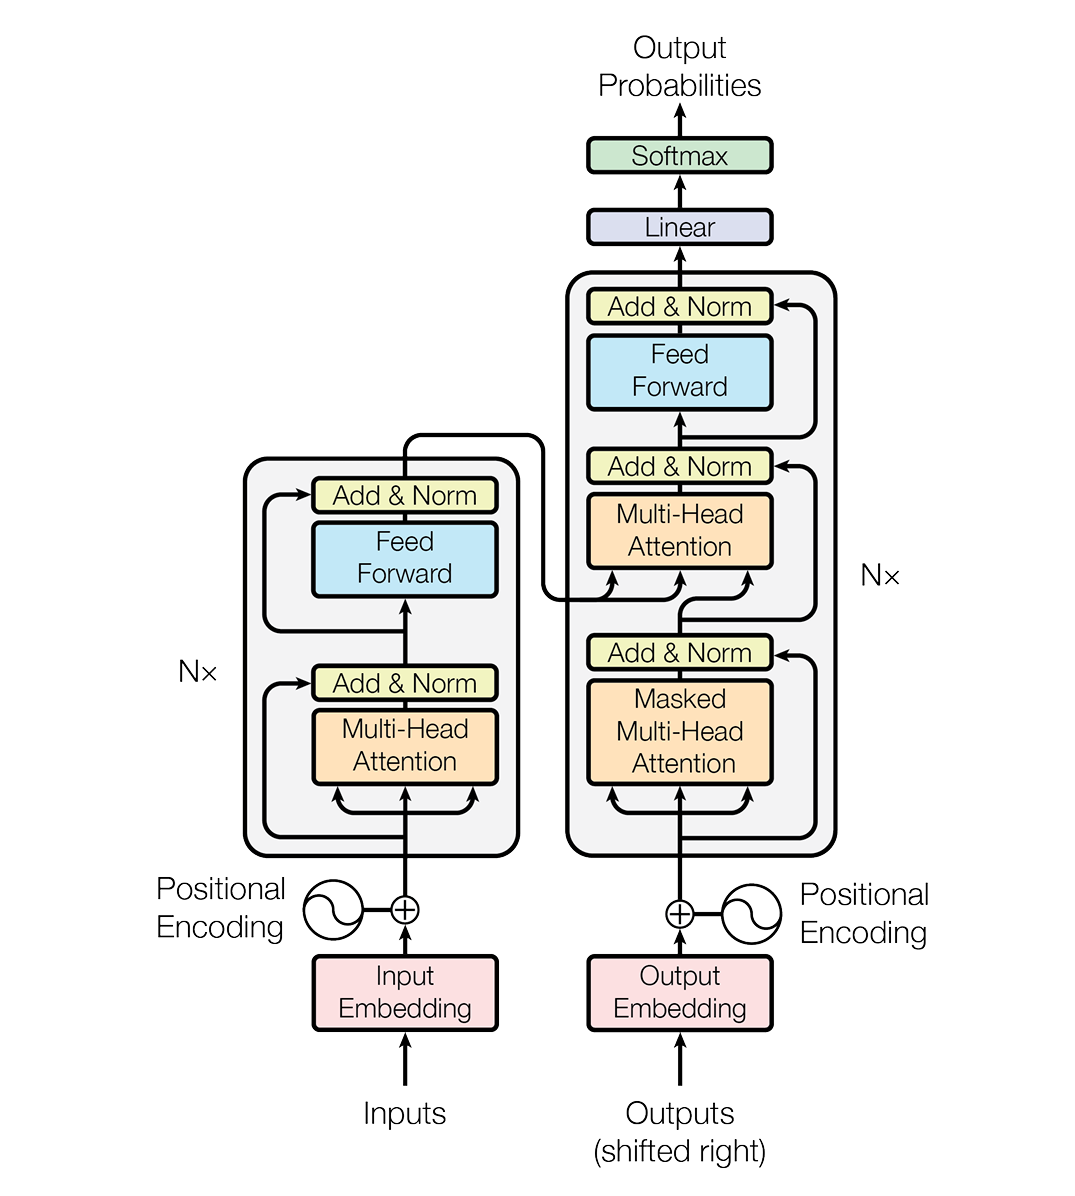
\includegraphics[width=0.5\linewidth]{images/transformers}
	\caption{Architecture of Transformers \cite{vaswani2023attention}}
	\label{fig:transofrmers}
\end{figure}


The main components of a transformer architecture include an encoder and a decoder. The encoder processes the input text and extracts features through multiple layers of self-attention mechanisms and feed-forward neural networks. The decoder generates the output text from the encoded representation, also utilizing self-attention mechanisms and attending to previously generated output tokens.

Self-attention is a crucial mechanism in transformers, enabling the model to weigh the contextual relevance of words in the input text. It computes a weighted sum of input embeddings based on the similarity between words and query, key, and value vectors, allowing the model to capture long-range dependencies and contextual relationships.

To address the absence of inherent word order in transformers, positional encoding is used to inject positional information into the input text. This is achieved by adding sinusoidal functions to the input embeddings, encoding the position of each word in the sequence.

Transformers have several advantages, including their ability to model long-range dependencies in text, which is challenging for traditional recurrent models. They have achieved state-of-the-art results in various NLP tasks and are widely used in many NLP applications. Popular transformer-based models include BERT, GPT-2, and Bloom, among others.\cite{tunstall2022natural} \cite{lin2021survey}



\subsection{BLOOM: A 176B-Parameter Open-Access Multilingual Language Model}

BLOOM \cite{workshop2023bloom}, a formidable multilingual language model with 176 billion parameters, is the collaborative result of hundreds of researchers. Trained on a carefully selected dataset called ROOTS, consisting of 46 natural languages and 13 programming languages, BLOOM shows versatility and robust performance. It uses a causal decoder-only strategy, BLOOM went through multitasking prompted fine-tuning to enhance its zero-shot task generalization capabilities, achieving competitive performance across various benchmarks.

The ROOTS corpus compromise of carefully selected Data from diverse sources, including NLP datasets, PDF files, online entries, and archives, that was compiled through community activities and hackathons. A quality filtering approach, which included the elimination of non-natural language content and personally identifiable information (PII), assured data integrity and privacy. The ROOTS corpus included a total of 46 natural languages and 13 programming languages. The natural languages included English, French, Spanish, Arabic, Simplified Chinese and many more. However German is not one of these languages.

The model architecture incorporates significant modifications to the Transformer framework, enhancing its capabilities:

\begin{enumerate}
    \item Multi-Head Attention: BLOOM incorporates multi-head attention, allowing simultaneous focus on different segments of the input stream. This adaptation enhances the model's capacity to capture intricate links and dependencies within the data.
    \item Softmax Activation: Softmax activation components are integrated into BLOOM's architecture, normalizing attention weights during the attention process. This ensures proper weighting for each input component.
    \item Layer Normalization (LN): BLOOM utilizes layer normalization to balance activations within each layer, contributing to improved overall performance and stabilized training.
    \item Key-Query Product: The attention mechanism employs the key-query product operation, enhancing relevance calculation between query and key vectors during the attention process.
    \item MLP (Multi-Layer Perceptron): BLOOM's design incorporates MLP layers for non-linear transformations, enabling the model to capture intricate patterns in the data.
    
\end{enumerate}

For BLOOM's text generation evaluation, metrics include ROUGE-2, ROUGE-1, and Levenshtein distance, assessing the model's performance in terms of n-gram overlap and string similarity.

These thoughtful modifications were strategically implemented to augment BLOOM's functionality, empowering it to proficiently handle a diverse array of tasks. Through a blend of collaborative effort and technological innovation, BLOOM stands as a testament to the evolving landscape of multilingual language models.

\subsection{Transfer learning}
Transfer learning is a machine learning strategy that uses information learned from a source domain and task to improve the learning process of a related target domain task. The technique may be used to overcome the resource-intensive demands of deep learning models, allowing for more efficient model training and increased performance. It can be used for a variety of NLP tasks, including question answering, sentiment analysis, and translation, demonstrating its versatility.\cite{alyafeai2020survey}

The two main techniques to transfer learning are to use a pre-trained model or to develop a new model. The former employs a pre-trained source model, and it is fine-tuned to fit the target model. This strategy is especially beneficial when the source and target tasks are comparable. The latter technique involves creating a new model for the target task based on insights learned from a previous task. For example, if there is insufficient data to recognize trucks and buses, a model originally built to detect automobiles can serve as a starting point, offering a foundation for additional refining and training.\cite{alyafeai2020survey}

\subsection{BLOOM-CLP German}\label{german-bloom}

In this thesis, we apply a specific model in order to use LLMs for German text generation: the German fine-tuned BLOOM. This monolingual German language model based on BLOOM-7b1 trained on 50 billion German tokens, is the outcome of the CLP-Transfer method, an innovative technique. The CLP-Transfer method was introduced in \cite{Ostendorff2023clp}

The motivation behind CLP-Transfer lies in overcoming limitations inherent in Transformer language models pre-trained in English, which may hinder their adaptability to other languages. Addressing this challenge, the proposed method extends the applicability of pre-trained models to different languages and model sizes. It employs a cross-lingual transfer approach, transferring knowledge from a source language (in this case, English) to a target language (German) using a smaller model architecture.

The CLP-Transfer technique outperformed the baselines in terms of training efficiency and downstream task performance, according to the results of the studies. CLP-Transfer obtained the same validation perplexity (PPL) as from-scratch training in the first experiment but with just 50\% of the used tokens. CLP-Transfer was superior to from-scratch training in the second experiment, achieving a lower PPL after training on 20\% of the tokens. CLP-Transfer efficiency benefits were considerably greater when applied to a model with 6.4B parameters vs a model with 1.5B parameters. Furthermore, when tested on downstream tasks, the CLP-Transfer models did better than smaller models and were on par with or better than the random baseline.


\subsection{BERT: Bidirectional Encoder Representations from Transformers}

BERT \cite{devlin2019bert}, or Bidirectional Encoder Representations from Transformers, stands as a revolutionary advancement in NLP. Developed by Google, BERT excels in understanding the nuances of language by considering context from both directions—left to right and right to left. Its architecture, based on transformers, enables the model to capture intricate relationships between words in a given context.

Unlike traditional models that process text in a unidirectional manner, BERT's bidirectional approach allows it to grasp the full context of each word within a sentence. This contextual understanding empowers BERT to generate more accurate and contextually relevant responses in various NLP tasks, such as question answering and text classification.

The training process involves exposing BERT to vast amounts of diverse language data, allowing it to learn the contextual intricacies of words and phrases. This pre-training phase is followed by fine-tuning specific tasks and tailoring the model to excel in various applications.

BERT's significance lies in its ability to comprehend the subtleties of language, making it a valuable tool in applications where context and nuanced understanding are crucial. Its impact resonates across diverse domains, showcasing the transformative power of bidirectional language modeling in the field of NLP.

\subsection{GPT2}\label{gpt2}

GPT-2, or Generative Pre-trained Transformer 2, is a large language model trained on a diverse web page dataset. Its evaluation across NLP tasks, including summarization, reading comprehension, question answering, and translation, showcases versatile capabilities. In summarization tasks, particularly on the CNN and Daily Mail dataset, GPT-2 employs top-k random sampling for abstractive summaries, yielding preliminary results based on quantitative metrics. Nevertheless, it demonstrates competitive performance in reading comprehension and question answering, achieving state-of-the-art results in a zero-shot setting. GPT-2's potential for multitask learning is highlighted, emphasizing the importance of model capacity. While promising, its practical applications, especially in summarization, remain limited. The model exhibits memorization behavior and shows promise in tasks like English-French translation, hinting at its broader potential in various NLP applications. However, the challenge of adapting GPT-2, originally released for English, to other languages poses a difficulty for users seeking text generation in different languages.\cite{radford2019language}

\subsubsection{GPT2-wechsel-german}

The WECHSEL method, which uses multilingual static word embeddings to efficiently transfer pretrained language models to new languages, is discussed in the paper\cite{minixhofer-etal-2022-wechsel}. Specifically, the authors conducted experiments to transfer the English GPT-2 model to various languages, including French, German, Chinese, Swahili, and four low-resource languages. They compared the performance of the transferred models to those initialized using other methods such as FullRand and TransInner using Language Modelling Perplexity on a held-out set. The results showed that across all languages and tasks, GPT-2 models initialized with WECHSEL consistently outperformed models initialized with other methods, achieving high performance with significantly fewer training steps.

\subsection{Mistral 7B}\label{mistral}
Mistral 7B, with 7 billion parameters, surpasses larger models on diverse benchmarks, emphasizing superior performance and computational efficiency. Its attention mechanisms, grouped-query attention (GQA) and sliding window attention (SWA), expedite inference and handle long sequences effectively. \cite{jiang2023mistral}

Released under the Apache 2.0 license, Mistral 7B prioritizes accessibility, enabling easy deployment and fine-tuning across various platforms. Notably, it excels in instruction fine-tuning, particularly in generating chat responses, outperforming models like Llama 2 13B in evaluations.\cite{jiang2023mistral}

To enhance ethical use, Mistral employs system prompting and self-reflection, providing mechanisms for controlled responses and content moderation in front-facing applications. Overall, Mistral 7B stands out as an efficient, adaptable language model with a focus on performance and responsible AI practices.\cite{jiang2023mistral}

\subsubsection{EM German}
EM German is a model family built on the Llama2, Mistral, and LeoLM architectures and trained on a large dataset of different instructions in the German language. These models are particularly designed for German text, displaying proficiency in interpreting, creating, and interacting with German information. Variants based on 7b, 13b, and 70b Llama-2, Mistral, and LeoLM models are available on hugging Face platform\footnote{Check \url{https://huggingface.co/jphme/em_german_mistral_v01}}.\cite{jphme2023}

\section{Prompts in LLMs}

In the realm of NLP, a prompt serves as the instructive input or query given to a language model to elicit a specific response. Think of it as the guiding question or statement that initiates the model's understanding and generates relevant content. The effectiveness of a prompt lies in its ability to clearly convey the user's intent, guiding the model to produce desired outputs. In NLP tasks such as text generation or question answering, crafting well-structured and contextually relevant prompts is pivotal for harnessing the full potential of language models. A carefully designed prompt acts as the bridge between human instruction and machine-generated language, influencing the quality and coherence of the model's responses.

\subsection{Prompt Engineering}

Prompt engineering plays a critical role in optimizing the performance of LLMs like BLOOM. It involves the deliberate construction of input prompts to guide the model's language generation process. In the context of this research, prompt engineering revolves around the inclusion of key features such as product details and category descriptions.

The paper \cite{gaoprompt} focuses on the strategies in prompt engineering tailored for LLMs. The guide emphasizes the importance of well-crafted prompts in a variety of applications, ranging from recipe generation to code writing. including using few-shot prompting with balanced examples, using Chain of Thought prompting for complex tasks, leveraging LLMs' coding abilities, and utilizing role prompting for specialized content are some of the strategies that are investigated.

In Chain of Thought prompting, complex tasks are simplified, similar to how we solve problems as humans. The technique provides a step-by-step explanation of a complex problem, allowing the LLM to solve new problems based on the reasoning provided.

The role prompting theory suggests that LLMs who are prompted as experts in a particular field are more likely to produce better results. In this way, they are able to focus and generate text in a specific creative style.

The significance of prompt engineering lies in its ability to shape the model's understanding of the input and guide it toward generating coherent and contextually relevant outputs. Crafting well-structured prompts is essential, as it influences how the model processes and interprets the given information. This strategic approach not only ensures accuracy in language generation but also enhances the adaptability of LLMs to various input scenarios.




\subsection{Zero/one/few-shot prompting}

Zero-shot, one-shot, and few-shot prompting are innovative techniques employed in prompt engineering for LLMs such as BLOOM. This technique provides LLMs with examples of the desired outputs, guiding them in producing the desired results. To avoid bias, it is critical to provide diverse and balanced examples. \cite{chen2023unleashing}

\begin{itemize}
    \item Zero-Shot prompting: In zero-shot prompting, the model is provide with no examples to evaluate it's understanding of the underlying task. 
    \item One-Shot prompting: One-shot prompting involves providing a single example to a LLM for it to learn from. This approach assesses the model's capacity to grasp information quickly and make accurate predictions based on minimal exposure.
    \item Few-Shot prompting: Few-shot prompting involves providing the model with small set of examples per task or category. This method allows the model to leverage a modest amount of task-specific information, enhancing its ability to generate contextually relevant and accurate language outputs.
\end{itemize}

The choice between one-shot and few-shot prompting is determined by the task's complexity and the model's capability. One-shot prompting may be sufficient for simple tasks or highly capable models. Few-shot prompting, on the other hand, can provide additional context and guidance for more complex tasks or less capable models, thereby improving the model's performance. It should be noted that, while examples can help guide the model, they do not always improve its performance. In some cases, zero-shot prompts outperform few-shot prompts, implying that the role of few-shot examples may be more about guiding the model to recall a previously learned task rather than teaching it a new task.

These techniques allow LLMs to grasp new tasks and generate more accurate and contextually relevant responses based on the given examples, offering flexibility in adapting to user needs and scenarios.

\section{Challanges}

\subsection{Evaluating Text Generated by LLMs}

Assessing the quality of text generated by LLMs involves a diverse set of evaluation metrics that examine different aspects of linguistic performance. One crucial metric is readability, with scores like Flesch Reading Ease providing insights into the ease of comprehension. Flesch Reading Ease considers factors like sentence length and syllable count, assigning a score that reflects the text's readability. A higher score indicates more accessible content.

Using the following formula, the Flesch Reading Ease score for English can be determined: 
$ FRE = 206.835 - 84.6 * WL - 1.015 * SL $. WL comes from the ratio of syllables in the text to words in the text, and SL from the ratio of words to sentences in the text. The calculations are based on the frequency of syllable lengths, phrase lengths, and word lengths in English.\cite{RyteWiki}


On the other hand, BLEU (Bilingual Evaluation Understudy) is a metric commonly used for machine-generated text, assessing the similarity between generated text and reference text. BLEU operates by comparing n-grams in the generated and reference text, providing a quantitative measure of linguistic overlap and fluency.\cite{Bleu}

Information extraction metrics, such as Named Entity Recognition (NER), focus on identifying and classifying entities (e.g., names, locations) in generated text. NER assesses the model's ability to accurately recognize and categorize specific information, essential for tasks where precise identification is paramount.\cite{Ner}

The paper \cite{liu2023trustworthy} emphasizes the crucial task of evaluating the alignment of LLMs to ensure their trustworthiness in various applications. It provides a comprehensive survey of key dimensions for assessing LLM trustworthiness, including reliability, safety, fairness, resistance to misuse, explainability and reasoning, adherence to social norms, and robustness. Challenges in evaluating LLM alignment are discussed alongside case studies and measurement results to support the findings. The goal is to offer valuable insights and guidance to practitioners for achieving reliable and ethically sound deployment of LLMs. Additionally, the issue of misinformation generated by LLMs is explored, highlighting the challenges in detecting and mitigating false or inaccurate information. Approaches for evaluation include text similarity metrics, truthfulness classifiers, and human evaluation. Despite ongoing research, a foolproof strategy to completely eliminate misinformation in LLMs is currently lacking. Similarly, the document delves into the concept of hallucination in LLMs, where nonsensical or unfaithful content is generated. The causes and evaluation methods for hallucination are discussed, and mitigating strategies involve improving training data quality, using different rewards in reinforcement learning, and leveraging external knowledge bases.

Additionally, This paper \cite{liu2023geval} introduces the G-EVAL framework for NLG evaluation using LLMs with chain-of-thoughts and a form-filling paradigm. G-EVAL outperforms previous metrics, achieving a higher correlation with human judgments in tasks like text summarization and dialogue generation. The framework is experimentally validated using GPT-4 and showcases effectiveness in assessing NLG systems for creativity and diversity.

Furthermore, efforts to assess LLMs as agents in interactive settings are presented in the paper \cite{liu2023agentbench} introducing AgentBench. This comprehensive benchmark employs metrics such as Success Rate, Element Accuracy, Action F1, Step Success Rate, and Task Success Rate across diverse interactive environments, emphasizing the need for improvements in open-source LLMs.

Lastly, the paper \cite{li2023static} introduces the DeepEval framework, addressing limitations in existing LLM evaluation methods. This novel deep interaction-based approach demonstrates effectiveness in evaluating LLMs in real-world scenarios across various tasks, emphasizing the need for a dynamic evaluation approach in complex environments.

These metrics collectively contribute to a comprehensive evaluation framework, allowing researchers to assess the fluency, coherence, and informativeness of text generated by LLMs. While readability scores and BLEU capture aspects of linguistic quality, information extraction metrics delve into the model's ability to comprehend and convey specific details—a crucial dimension in evaluating the practical applicability of language models.

\subsection{Text Generation with LLMs in German Language}

Generating text with LLMs, such as by BLOOM, poses considerable challenges attributed to the intricate nature of language tasks and the distinct characteristics of diverse languages. The inherent complexity arises from navigating the grammar rules, vocabulary subtleties, and cultural nuances that LLMs must capture and reproduce during the text generation process.

Mark Twain's humorous exploration of German \cite{twain1880awfulgerman}, categorized as a Category 2 language in the FSI ranking \cite{Kenny}, sheds light on the difficulties learners face, as the language is much more difficult to learn for English speakers than other Category 1 languages like French and Spanish. Twain's humorous commentary underscores the intricacies of German grammar, involving noun genders, adjective declensions, and separable verbs, resonating with language learners grappling with the challenges of this Category 2 language.

In the context of text generation challenges specific to German, linguistic intricacies and the limited availability of training data create hurdles. LLMs, like Bloom or LLaMA, may not adequately include German in their training datasets or only include it minimally. Given the compound words, grammatical structures, and contextual dependencies unique to German, a nuanced understanding is crucial but may be hindered by insufficient data. This scarcity of diverse German-language datasets further complicates the models' capacity to generate culturally appropriate and contextually relevant text.

German's classification as a Germanic rather than a Romance language implies substantial divergences in linguistic structure from languages like French and Spanish. LLMs primarily trained on Romance languages might face difficulties adapting to German's unique features, potentially affecting their performance in text generation tasks due to syntactic and semantic disparities. Recognizing these distinctions becomes pivotal for optimizing LLMs, ensuring accurate and contextually relevant language processing for German and similar non-Romantic languages.






